\documentclass[12pt]{article}

\usepackage[utf8]{inputenc}
\usepackage[spanish]{babel}
\usepackage{enumerate}
\usepackage{amsmath}
\usepackage{txfonts}
\usepackage{graphicx}
\usepackage{keystroke}
\usepackage{color}
\usepackage[colorlinks = true,
linkcolor = green,
urlcolor = blue,
citecolor = yellow,
anchorcolor = brown]{hyperref}
\usepackage{listings}
\usepackage{alltt}
\usepackage{multicol}

\definecolor{mygreen}{rgb}{0,0.6,0}
\definecolor{mygray}{rgb}{0.5,0.5,0.5}
\definecolor{mymauve}{rgb}{0.58,0,0.82}

\lstset{ %
  backgroundcolor=\color{white},   % choose the background color; you must add \usepackage{color} or \usepackage{xcolor}
  basicstyle=\footnotesize,        % the size of the fonts that are used for the code
  breakatwhitespace=false,         % sets if automatic breaks should only happen at whitespace
  breaklines=true,                 % sets automatic line breaking
  captionpos=b,                    % sets the caption-position to bottom
  commentstyle=\color{mygreen},    % comment style
  deletekeywords={...},            % if you want to delete keywords from the given language
  escapeinside={\%*}{*)},          % if you want to add LaTeX within your code
  extendedchars=true,              % lets you use non-ASCII characters; for 8-bits encodings only, does not work with UTF-8
  frame=single,                    % adds a frame around the code
  keepspaces=true,                 % keeps spaces in text, useful for keeping indentation of code (possibly needs columns=flexible)
  keywordstyle=\color{blue},       % keyword style
  language=Octave,                 % the language of the code
  morekeywords={*,...},            % if you want to add more keywords to the set
  numbers=left,                    % where to put the line-numbers; possible values are (none, left, right)
  numbersep=5pt,                   % how far the line-numbers are from the code
  numberstyle=\tiny\color{mygray}, % the style that is used for the line-numbers
  rulecolor=\color{black},         % if not set, the frame-color may be changed on line-breaks within not-black text (e.g. comments (green here))
  showspaces=false,                % show spaces everywhere adding particular underscores; it overrides 'showstringspaces'
  showstringspaces=false,          % underline spaces within strings only
  showtabs=false,                  % show tabs within strings adding particular underscores
  stepnumber=2,                    % the step between two line-numbers. If it's 1, each line will be numbered
  stringstyle=\color{mymauve},     % string literal style
  tabsize=2,                       % sets default tabsize to 2 spaces
  title=\lstname                   % show the filename of files included with \lstinputlisting; also try caption instead of title
}

\newcommand{\noterm}[1]{\color{blue} \langle #1 \rangle \color{blue}}
\newcommand{\produce}{\color{red} \coloneqq \color{red}}
\newcommand{\alter}{\color{red} \mid \color{red}}
\newcommand{\catterm}[1]{\color{magenta} \text{#1} \color{magenta}}
\newcommand{\term}[1]{\color{cyan} \text{#1} \color{cyan}}
\newcommand{\openopt}{\color{black} \text{[} \color{black}}
\newcommand{\closeopt}{\color{black} \text{]} \color{black}}
\newcommand{\severals}{\color{black} \ldots \color{black}}

\newcounter{ejercicio}
\newcommand{\ejercicio}{\stepcounter{ejercicio}%
  \paragraph\noindent\textbf{Ejercicio \theejercicio.\hspace{4pt}}}

\newcounter{problema}
\newcommand{\problema}{\stepcounter{problema}%
  \paragraph\noindent\textbf{Problema \theproblema.\hspace{4pt}}}
\newcommand{\WindowsLogo}{\raisebox{-0.1em}{%
    \includegraphics[height=0.8em]{../../imagenes/Windows_3_logo_simplified}}}
\newcommand{\WinKey}{\keystroke{\WindowsLogo}}

\newcommand{\Subversion}{\href{https://subversion.apache.org/}{subversion}}
\newcommand{\Riouxsvn}{\href{https://riouxsvn.com/}{Riouxsvn}}

\title{Evaluación Cursos[1,2] de Scala\\Calculadora de Naturales Resta}
\date{23 de Septiembre 2021}
\author{EPAM Latam - S4N Campus}
%\institute{S4N}

\begin{document}
\maketitle

\section{Preliminares}
\label{sec:preliminares}

\begin{enumerate}
\item Cree un repositorio en \href{https://github.com}{GitHub} con el nombre \texttt{$<$emailusuario$>$-calnatsuma}. Donde \texttt{$<$emailusuario$>$} es el nombre de usuario en el su email de la compañía. Por ejemplo el nombre del repositorio de \texttt{juancardona@seven4n.com} sería \texttt{juancardona-calnatresta}.
\item Clone el repositorio en un directorio de trabajo.
\item Abra dicho directorio y pueble con la estructura de directorios que se observa \ref{fig:dir}.
  \begin{figure}[h]
    \centering
    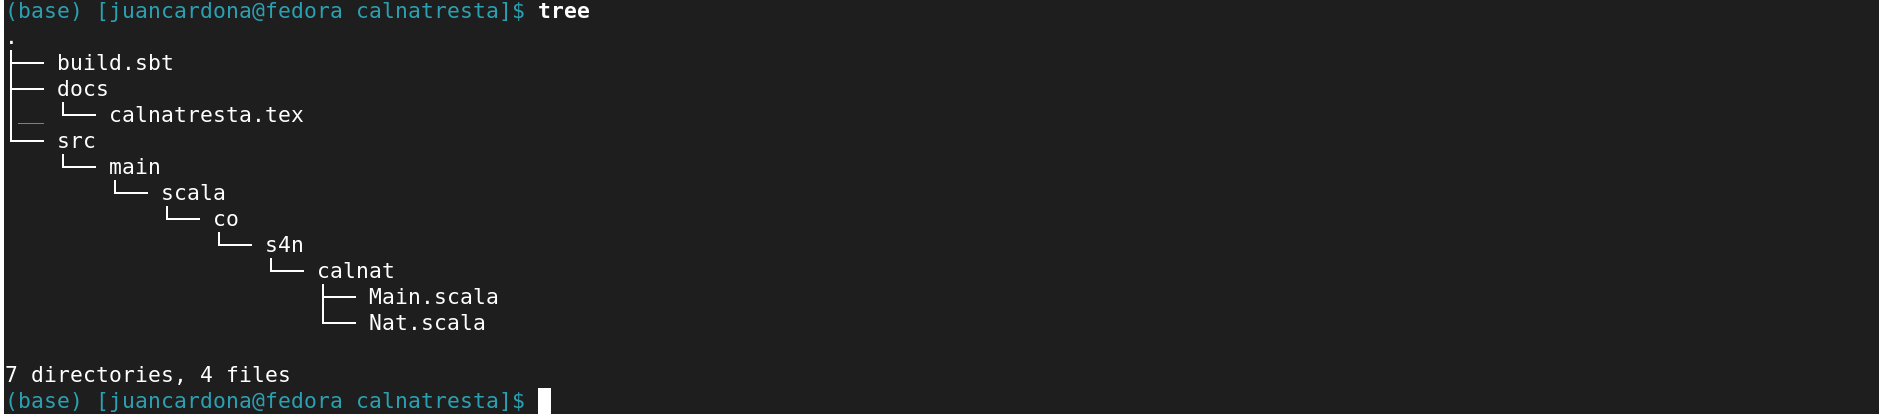
\includegraphics[width=10cm,height=10cm]{../../../imagenes/jerarquia-calnatresta.png}
    \caption{Estructura de directorios}
    \label{fig:dir}
  \end{figure}

\end{enumerate}

\section{Definición de tipos algebraicos los Naturales}
\label{sec:definicio-de-tipos}

Los \href{https://es.wikipedia.org/wiki/N%C3%BAmero_natural}{números naturales} pueden ser definidos como un tipo de dato algebraico. Donde el caso base se tiene el \texttt{Cero} y el caso recursivo es el sucesor de un natural.

\subsection{Definición de Naturales en Scala}
\label{sec:def-naturales}

\begin{lstlisting}[language=Scala]
package co.s4n.calnat

trait Nat
case class Cero() extends Nat
case class Suc(nat:Nat) extends Nat
\end{lstlisting}

Donde \texttt{Nat} es el tipo. \texttt{Cero} y \texttt{Suc} son los constructores de valores.

Una posible iteracción con los naturales se puede hacer así  para construir diferentes valores.

\begin{alltt}
scala> val cero = Cero
val cero: co.s4n.calnat.Cero = Cero
scala> val uno = Suc(Cero)
val uno: co.s4n.calnat.Suc = Suc(Cero)
scala> val dos = Suc(Suc(Cero))
val cero: bco.s4n.calnat.Suc = Suc(Suc(Cero))
\end{alltt}

\subsection{Coincidencia de patrones en los Naturales}
\label{sec:pat-nat}

La función \texttt{esCero} nos muestra como implementar la coincidencia de patrones en los naturales.

\begin{lstlisting}[language=Scala]
def esCero(nat:Nat):Boolean = nat match {
   case Cero()   => true
   case Suc(nat) => false
}
\end{lstlisting}

\section{Proyecto a implementar}
\label{sec:problema-resolver}

En el archivo \texttt{Main} debe tener implementar el objeto \texttt{Main} como lo hizo anteriormente cuando utilizo \texttt{sbt}.

El esqueleto del Main se muestra a continuación:

\begin{lstlisting}[language=Scala]
package co.s4n.calnat

import scala.io.StdIn

object Main extends App {
  def leerInt(prompt:String):Int = {
    val s = StdIn.readLine(prompt)
    s.toInt
  }
  def esCero(nat:Nat) = nat match {
    case Cero()   => true
    case Suc(nat) => false
  }
  def esMayorIgual(nat1:Nat,nat2:Nat):Boolean = nat1 match {
    case Cero() => nat2 match {
      case Cero() => true
      case _      => false
    }
    case Suc(pnat) => nat2 match {
      case Cero() => true
      case Suc(snat) => esMayorIgual(pnat,snat)
    }
  }
  def conIntANat(i:Int):Nat = ???
  def imprimirNat(nat:Nat):String = ???
  def restaNat(nat1:Nat,nat2:Nat):Nat = ???
  ...
}
\end{lstlisting}

Usted debe implementar los siguientes métodos:
\begin{itemize}
\item \texttt{conIntANat} convierte un entere a un valor de tipo Natural (\texttt{Nat}).
\item \texttt{imprimirNat} imprime un Natural siguiendo su estructura.
\item \texttt{restaNat} toma dos naturales \texttt{nat1} \texttt{nat2} y realiza una resta entre ellos. \textbf{Nota.} Todo el trabajo
  debe ser hecho en la estructura de los naturales.
\end{itemize}

Un vez implementado los anteriores métodos los utiliza para implementar el siguiente programa principal.

\begin{quote}
  El programa lee dos números enteros y cada uno de ellos los convierte a \emph{Naturales} (\texttt{Nat}) cada uno de ellos es
  restado utilizando \texttt{restaNat} y el resultado final lo imprime utilizando \texttt{imprimirNat}.
\end{quote}

Los valores enteros se suponen que son enteros positivos, \emph{no se hará verificación alguna}.

Una iteración de su programa \emph{podría} en la que se resta dos valores:

{\footnotesize
\begin{verbatim}
(base) [juancardona@fedora calnatresta]$ sbt run 
[info] welcome to sbt 1.4.2 (AdoptOpenJDK Java 11.0.9)
[info] loading project definition from /home/juancardona/Workbench/s4n_scala_synch_course/proyectos/calnatresta/project
[info] loading settings for project calnatresta from build.sbt ...
[info] set current project to calnatresta (in build file:/home/juancardona/Workbench/s4n_scala_synch_course/proyectos/calnatresta/)
[info] compiling 1 Scala source to /home/juancardona/Workbench/s4n_scala_synch_course/proyectos/calnatresta/target/scala-2.12/classes ...
[info] done compiling
[info] running co.s4n.calnat.Main 
Leer primer entero 10
Leer segundo entero 4
Suc(Suc(Suc(Suc(Suc(Suc(Cero))))))
[success] Total time: 7 s, completed 23/09/2021, 9:43:55 a. m.
(base) [juancardona@fedora calnatresta]$ 
\end{verbatim}
}

Observe que para la salida de la suma de \texttt{10 - 4} se obtiene:

\begin{verbatim}
Suc(Suc(Suc(Suc(Suc(Suc(Cero))))))
\end{verbatim}

El número de \texttt{Suc} establece el resultado.

Otra interacción con el programa ocurre así:

\begin{verbatim}
(base) [juancardona@fedora calnatresta]$ sbt run
[info] welcome to sbt 1.4.2 (AdoptOpenJDK Java 11.0.9)
[info] loading project definition from /home/juancardona/Workbench/s4n_scala_synch_course/proyectos/calnatresta/project
[info] loading settings for project calnatresta from build.sbt ...
[info] set current project to calnatresta (in build file:/home/juancardona/Workbench/s4n_scala_synch_course/proyectos/calnatresta/)
[info] running co.s4n.calnat.Main 
Leer primer entero 9
Leer segundo entero 10
No se puede hacer la operacion
[success] Total time: 3 s, completed 23/09/2021, 9:59:34 a. m.
(base) [juancardona@fedora calnatresta]$ 
\end{verbatim}
% \section{Bibliografía}
% \label{sec:bibliografia}
% \bibliographystyle{amsalpha}
% \bibliography{S4N_Git_Tutorial}

\end{document}

%%% Local Variables:
%%% mode: latex
%%% TeX-master: t
%%% End:
